%%%%%%%%%%%%%%%%%%%%%%%%%%%%%%%%%%%%%%%%%
% University Assignment Title Page 
% LaTeX Template
% Version 1.0 (27/12/12)
%
% This template has been downloaded from:
% http://www.LaTeXTemplates.com
%
% Original author:
% WikiBooks (http://en.wikibooks.org/wiki/LaTeX/Title Creation)
%
% License:
% CC BY-NC-SA 3.0 (http://creativecommons.org/licenses/by-nc-sa/3.0/)
% 
% Instructions for using this template:
% This title page is capable of being compiled as is. This is not useful for 
% including it in another document. To do this, you have two options: 
%
% 1) Copy/paste everything between \begin{document} and \end{document} 
% starting at \begin{titlepage} and paste this into another LaTeX file where you 
% want your title page.
% OR
% 2) Remove everything outside the \begin{titlepage} and \end{titlepage} and 
% move this file to the same directory as the LaTeX file you wish to add it to. 
% Then add \input{./title page_1.tex} to your LaTeX file where you want your
% title page.
%
%%%%%%%%%%%%%%%%%%%%%%%%%%%%%%%%%%%%%%%%%

%----------------------------------------------------------------------------------------
%	PACKAGES AND OTHER DOCUMENT CONFIGURATIONS
%----------------------------------------------------------------------------------------

\documentclass[12pt]{article}
\usepackage{graphicx}
\usepackage[utf8]{inputenc}  
\usepackage[T1]{fontenc} 
\usepackage[top=1cm,bottom=1cm,left=0.5cm,right=1.5cm,asymmetric]{geometry}
\usepackage{amsfonts}
\usepackage{graphicx}
\usepackage{algorithm}
\usepackage{algpseudocode}
\usepackage{amsmath}
\usepackage{caption}
\usepackage{subcaption}
\usepackage{float}
\usepackage{subfig}
\usepackage{fancyhdr}
\pagestyle{fancy}
\renewcommand{\footrulewidth}{1pt}
\fancyhead[R]{\textit{Master MVA : Simulation based learning}}
\fancyfoot[L]{\textit{}}
%\usepackage{unicode-math}
%\setmathfont{XITS Math}
%\setmathfont[version=setB,StylisticSet=1]{XITS Math}
\usepackage{array,multirow,makecell}
\setcellgapes{1pt}
\makegapedcells
\newcolumntype{R}[1]{>{\raggedleft\arraybackslash }b{#1}}
\newcolumntype{L}[1]{>{\raggedright\arraybackslash }b{#1}}
\newcolumntype{C}[1]{>{\centering\arraybackslash }b{#1}}

\pagestyle{fancy}
\renewcommand{\footrulewidth}{1pt}
\fancyfoot[L]{\textit{}}
\newcommand{\cond}{(x_i|x_{\pi_i})}

%\usepackage{caption}
%\usepackage{subcaption}


%\usepackage{unicode-math}
%\setmathfont{XITS Math}
%\setmathfont[version=setB,StylisticSet=1]{XITS Math}


%\geometry{hmargin=1.5cm,vmargin=2cm}   

\geometry{hmargin=2.5cm,vmargin=2cm}   
\begin{document}
	
	\section*{Homework 3 :  Part A}
	\section*{Oussama Ennafii \& Sammy Khalife}
	\subsubsection*{25/02/2015}
	
	\section*{Exercise 1}
	1. Let $\gamma \in \mathbb{N^*}$ and $X=\{1,..,6\}$. We consider the Hastings-Metropolis algorithm with target $\pi$ associated to the proposal distribution:
	$$q(x,.)=\mathcal{U}(\{X_n - \gamma, X_n-\gamma+1,..., X_n-1, X_n+1,...,X_n+\gamma\})$$~\\
	
	\begin{algorithm}
		\caption{Metropolis Hastings algorithm}\label{RS}
		Given one initial point in $x_0 \in X$~\\
		for n=1:N~\\
		-Generate $Y_n \sim q(x_n,.) $~\\
		-$X_{n+1}=Y_n$ with probability $\alpha(X_n, Y_n)$~\\
		and $X_{n+1}=X_{n}$ with probability $1-\alpha(X_n, Y_n)$.~\\
		end~\\
	\end{algorithm}
	~\\
	Since $\forall x \in X, \forall y \in X, q(x,y)=\frac{1}{2\gamma}$, the acceptance ratio is equal to 
	$$
	\alpha(x,y) =
	\begin{cases}
	1 \wedge \frac{\pi(y)}{\pi(x)} & \text{if \quad }  y \in X\\
	0 & \text{otherwise}
	\end{cases}
	$$
	To avoid technical discussions, we will consider the extended distribution $\pi$ on $\mathbb{Z}$, with $\pi(k)=0$ if $k \notin X$ so that :
	$$
	\alpha(x,y) = 1 \wedge \frac{\pi(y)}{\pi(x)} 
	$$
	~\\
	~\\
	And the transition kernel is equal, for $y \neq x$ to:
	\begin{eqnarray*}
		p(x,y)&=& q(x,y)\alpha(x,y)\\
		&=& \frac{1}{2\gamma} ( 1 \wedge \frac{\pi(y)}{\pi(x)} ) \\ 	
	\end{eqnarray*}
	and : 
	\begin{eqnarray*}
		p(x,x)&=& 1-\sum_{y \neq x}q(x,y)\alpha(x,y) 	
	\end{eqnarray*}
	First :
	\begin{eqnarray*}
		p(x,y \neq x) & = & \frac{1}{2\gamma}(1 \wedge \frac{\pi(y)}{\pi(x)})\\
		& \geq & \frac{1}{2\gamma }(1 \wedge \frac{\pi(y)}{\max_x \pi(x)})\\
		& = &  \frac{\pi(y)}{2\gamma \max_x \pi(x)}\\
		& \geq & 	 \frac{\pi(y)}{2\gamma}	 
	\end{eqnarray*}
	The third equality is due to $\frac{\pi(y)}{\max_x \pi(x)} \leq 1 $.
	The fourth inequality is due to $max_x \pi(x) \leq 1$.~\\
	~\\
	Second, 
	\begin{eqnarray*}
		p(x,x)&=& 1-\sum_{y \neq x}q(x,y)\alpha(x,y) \\
		&=& q(x,x)+\sum_{y \neq x}q(x,y) -\sum_{y \neq x}q(x,y)\alpha(x,y)\\
		&=& q(x,x) + \sum_{x \neq y}q(x,y)(1-\alpha(x,y))\\
		& \geq & q(x,x)\\
		& = & \frac{1}{2\gamma}\\
		& \geq & \frac{\pi(x)}{2\gamma} 
	\end{eqnarray*}
	The second inequality is obtained by upper bounding the sum terms by 1, and using $|X|=6$.
	Let $\boxed{\epsilon=\frac{1}{2\gamma}}$, then
	$$\forall x, \forall y \quad p(x,y) \geq \epsilon  \pi(y)$$
	which can be written in terms of subsets B of $X$ :
	$$\boxed{p(x,B) \geq \epsilon  \pi(B)}$$
	~\\
	2. Given the inequality written above, the algorithm satisfies the Doeblin condition. The Doeblin Lemma gives : $ \boxed{\Delta(P) \leq ( 1 - \epsilon )}$~\\
	~\\
	Given one initial distribution $\xi$, we have in the general case:
	$$||\xi P^n - \pi||_{TV} \leq (\Delta(P))^{ n } ||\xi-\pi||_{TV}$$
	which yields here :
	$$ \boxed{||\xi P^n - \pi||_{TV} \leq (1-\frac{1}{2\gamma})^{ n } ||\xi-\pi||_{TV}}$$~\\
	Where $\xi P^n$ is actually the distribution of $X_n$. We have geometric ergodicity~\\
	~\\
	3. Cf code for implementation.~\\
	The following error is computed with comparison of the numerical mean and the theoretical mean :  $\pi(1)=\frac{1}{2}$, $\pi(2)=\frac{2}{6}$, $\pi(3)=\frac{1}{24}$, $\pi(4)=\frac{1}{24}$, $\pi(5)=\frac{1}{24}$, $\pi(6)=\frac{1}{24}$, using the average of simulations (Monte Carlo method).~\\
	~\\
	$\gamma=1$,  $error=0.1440$.~\\
	$\gamma=4$ $error=0.0641$~\\
	$\gamma=50$ $error=0.1818$~\\
	~\\
	The large error for $\gamma50$ is not surprising since small values of $\gamma$ provide a better theoretical upper bound (cf 2). Here, we see that there is a trade off with regards of the value of $\gamma$. Small values will not promote the exploration of the set X which explains the bad convergence of the algorithm.
	\section*{Exercise 2}
	1. Let a family of transition matrices $$ P_t = \begin{bmatrix} t & (1-t) \\ (1-t) & t \end{bmatrix} $$~\\
	~\\
	The obvious invariant distribution is $\pi=\begin{bmatrix} \frac{1}{2} \\ \frac{1}{2} \end{bmatrix}$.
	~\\
	\textbf{Properties of this Markov Chain}~\\
	~\\
	Since $t \in ]0,1[$, the Markov Chain is obviously irreducible. ~\\
	~\\
	Since the coefficients $p_{1,1}$ and $p_{2,2}$ are strictly positive $(t > 0)$, all the states are aperiodic and then the chain is aperiodic.~\\
	~\\
	Finally, we will show that the chain is recurrent positive by considering $p^{(k)}_{i,i}$.~\\
	~\\
	The matrix can reduce itself to 
	$$D = \begin{bmatrix} 2t-1 & 0 \\ 0 & 1 \end{bmatrix} $$
	with $Q = \begin{bmatrix} 1 & -1 \\ 1 & 1 \end{bmatrix}$,
	$QDQ^{-1}=P_{t}$ and $P_{t}^{n}=QD^{n}Q^{-1}$,
	which gives : 
	$$P_{t}^{n} \begin{bmatrix} (2t-1)^{n}\frac{1}{2}+ \frac{1}{2} & -(2t-1)^{n}\frac{1}{2}+ \frac{1}{2} \\ -(2t-1)^{n}\frac{1}{2}+ \frac{1}{2} & (2t-1)^{n}\frac{1}{2}+ \frac{1}{2} \end{bmatrix} $$
	Then, $ \forall i \in \{0,1\}, \sum_{k \geq 0} p_{i,i}^{(k)} = +\infty$, and the chain is recurrent positive.
	There is convergence of the law of $X_n$ towards the invariant distribution independently of the initial distribution.~\\
	~\\
	2. Given the algorithm written $X_n$ depends only on $X_{n-1}$ and, $$\mathbb{P}(X_{n+1}=x | X_{n}=y)= P_{t_0}(y,x)\textbf{1}_{y=0}+P_{t_1}(y,x)\textbf{1}_{y=1}$$, then 
	
	$$P_{*}= \begin{bmatrix} t_0 & (1-t_1) \\ (1-t_0) & t_1 \end{bmatrix}$$
	Solving 
	$$ \pi^{*} P_{*} = \pi^{*} $$ 
	gives $\pi^{*}_1=\frac{\pi_2(t_1-1)}{t_0-1}$, and $\pi^{*}_1 + \pi^{*}_2 = 1 $ yields :
	$$\boxed{\pi^{*}_1 = \frac{t_1-1}{t_0+t_1 -2}}$$
	and
	$$\boxed{\pi^{*}_2 = \frac{t_0-1}{t_0+t_1-2}}$$
	The chain is obviously irreducible (each state is available from another since $t_0 \in ]0,1[$  and $t_1 \in ]0,1[$).
	
	\section*{Exercise 3}
	We choose for the numerical simulation the parameters:
	\begin{eqnarray*}
		N :&=&1000\\
		c :&=&2\\
		n_0 :&=&100
	\end{eqnarray*}
	
	1.  In figure ~\ref{nrwHM}, we see how the sequence $X^n_1$ varies too much and takes a long time to converge to the mean which is $0$ in this case. The second plot shows that the acceptance ratio also converges , slowly though, up to around $70\%$. So there is room to do better.
	\begin{figure}[H]
		\centering
		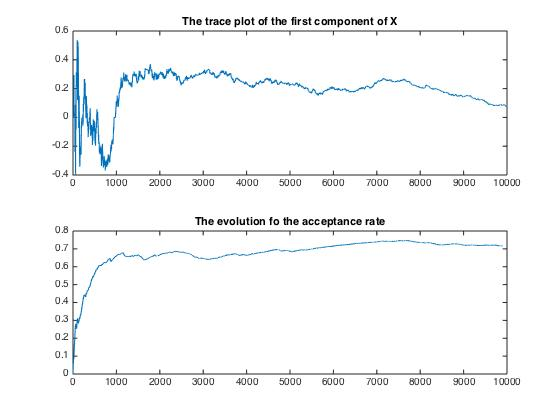
\includegraphics[scale=.5]{figures/nrwHM}
		\caption{The naive symmetric random walk Hastings-Metropolis chain}
		\label{nrwHM}
	\end{figure}
	~\\
	
	2.  In figure ~\ref{arwHM}, we see that the sequence $X_n$ converges abruptly to the mean after $n0$. The second plot shows that the acceptance ratio also converges rapidly up to around $100\%$. Further, we can see that the suboptimality factor depend on $n$ in $2$ ways. First, it varies a lot and stays strictly over $1$ (the optimal case). In the second phase, it starts decreasing very slowly to $1$.
	\begin{figure}[H]
		\centering
		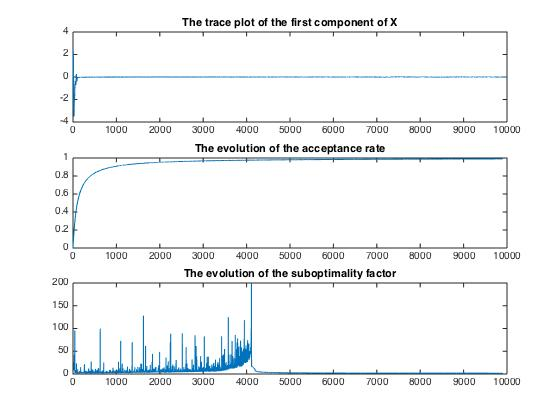
\includegraphics[scale=.5]{figures/arwHM}
		\caption{The adaptive symmetric random walk Hastings-Metropolis chain}
		\label{arwHM}
	\end{figure}
	~\\
	
	3. The suboptimality factor of the first algorithm is constant independent from $c$:
	
	$$n \mapsto d\frac{trace(\Gamma_{\pi} ^2) }{trace(\Gamma_{\pi})^2}>1$$
	
	The adaptive algorithm yields a sequence that adapts and thus convergences, slowly, to the optimal case. In conclusion, the adaptive random walk is much better than the naive one.
	
	\newpage
	\section*{Homework 3 :  Part B}
	\section*{Oussama Ennafii \& Sammy Khalife}
	\subsubsection*{10/03/2015}
	
	\section*{Step 1}
	~\\
	
	1. The equality is trivial: we just have to set $\vartheta=\theta$.\\
	
	The fact that $g(\vartheta)$ is always positive means that, to prove the equality $$ Q_{\gamma}(\vartheta,\theta)\geq (f+g)(\vartheta)$$, we just need to prove that:
	
	$$f(\vartheta)\leq f(\theta)+<\nabla f(\theta),\vartheta-\theta>+\frac{1}{2\gamma}\vert\vert \vartheta-\theta\vert\vert^2$$
	
	~\\
	
	2. Let $n \in \mathbb{N}$:
	
	\begin{eqnarray*}
		(f+g)(\theta_{n})&=& Q_{\gamma_{n+1}}(\theta_{n},\theta_{n})\\
								&\geq& Q_{\gamma_{n+1}}(\theta_{n+1},\theta_{n})\\ 
								&\geq& (f+g)(\theta_{n+1})
	\end{eqnarray*}
	The first inequality is the result of the definition $\theta_{n+1}$. The second comes from the first question.\\
	
	3. 
	
	
\end{document}